%-------------------------------------------------------------------------------
%	PACKAGES AND OTHER DOCUMENT CONFIGURATIONS
%-------------------------------------------------------------------------------

\documentclass{article}

% Packages
% Packages

% \usepackage{fancyhdr} % Required for custom headers
% \usepackage{lastpage} % Required to determine the last page for the footer
% \usepackage{extramarks} % Required for headers and footers
% \usepackage[usenames,dvipsnames]{color} % Required for custom colors
\usepackage{graphicx} % Required to insert images
% \usepackage{listings} % Required for insertion of code
% \usepackage{courier} % Required for the courier font
% \usepackage{dsfont} % For special math characters
% \usepackage{verbatim}

%\usepackage{amsmath, amssymb, bm} % For matrix notation
\usepackage[english]{babel}
\usepackage[paperwidth=8.5in,paperheight=11in,margin=1.0in]{geometry}
\usepackage{listings}
\usepackage{hyperref}
%\usepackage[cmex10]{amsmath, bm}
\usepackage{amsmath, bm}
\usepackage{blkarray}








% formatting
\pdfcompresslevel0

% ==============================================================================
% PYTHON
% ==============================================================================
\usepackage[utf8]{inputenc}

% Default fixed font does not support bold face
\DeclareFixedFont{\ttb}{T1}{txtt}{bx}{n}{12} % for bold
\DeclareFixedFont{\ttm}{T1}{txtt}{m}{n}{12}  % for normal

% Custom colors
\usepackage{color}
\definecolor{deepblue}{rgb}{0,0,0.5}
\definecolor{deepred}{rgb}{0.6,0,0}
\definecolor{deepgreen}{rgb}{0,0.5,0}

\usepackage{listings}

% Python style for highlighting
\newcommand\pythonstyle{\lstset{
language=Python,
basicstyle=\ttm,
otherkeywords={self},             % Add keywords here
keywordstyle=\ttb\color{deepblue},
emph={MyClass,__init__},          % Custom highlighting
emphstyle=\ttb\color{deepred},    % Custom highlighting style
stringstyle=\color{deepgreen},
frame=tb,                         % Any extra options here
showstringspaces=false,            % 
breaklines=true
}}


% Python environment
\lstnewenvironment{python}[1][]
{\pythonstyle\lstset{#1}
}
{}

% Python for external files
\newcommand\pythonexternal[2][]{{
\pythonstyle\lstinputlisting[#1]{#2}}}

% Python for inline
\newcommand\pythoninline[1]{{\pythonstyle\lstinline!#1!}}
% ==============================================================================
% ==============================================================================

% Margins
\topmargin=-0.45in
\evensidemargin=0in
\oddsidemargin=0in
\textwidth=6.5in
\textheight=9.0in
\headsep=0.25in

\linespread{1.1} % Line spacing

% Set up the header and footer
\pagestyle{fancy}
\lhead{\hmwkAuthorName} % Top left header
\chead{\hmwkClass\ (\hmwkClassInstructor\ \hmwkClassTime): \hmwkTitle} % Top center head
\rhead{\firstxmark} % Top right header
\lfoot{\lastxmark} % Bottom left footer
\cfoot{} % Bottom center footer
\rfoot{Page\ \thepage\ of\ \protect\pageref{LastPage}} % Bottom right footer
\renewcommand\headrulewidth{0.4pt} % Size of the header rule
\renewcommand\footrulewidth{0.4pt} % Size of the footer rule

\setlength\parindent{0pt} % Removes all indentation from paragraphs

%----------------------------------------------------------------------------------------
%	DOCUMENT STRUCTURE COMMANDS
%	Skip this unless you know what you're doing
%----------------------------------------------------------------------------------------

% Header and footer for when a page split occurs within a problem environment
\newcommand{\enterProblemHeader}[1]{\nobreak\extramarks{#1}{#1 continued on next page\ldots}\nobreak\nobreak\extramarks{#1 (continued)}{#1 continued on next page\ldots}\nobreak}

% Header and footer for when a page split occurs between problem environments
\newcommand{\exitProblemHeader}[1]{\nobreak\extramarks{#1 (continued)}{#1 continued on next page\ldots}\nobreak\nobreak\extramarks{#1}{}\nobreak}

\setcounter{secnumdepth}{0} % Removes default section numbers
\newcounter{homeworkProblemCounter} % Creates a counter to keep track of the number of problems

\newcommand{\homeworkProblemName}{}
\newenvironment{homeworkProblem}[1][Problem \arabic{homeworkProblemCounter}]{ % Makes a new environment called homeworkProblem which takes 1 argument (custom name) but the default is "Problem #"
\stepcounter{homeworkProblemCounter} % Increase counter for number of problems
\renewcommand{\homeworkProblemName}{#1} % Assign \homeworkProblemName the name of the problem
\section{\homeworkProblemName} % Make a section in the document with the custom problem count
\enterProblemHeader{\homeworkProblemName} % Header and footer within the environment
}{\exitProblemHeader{\homeworkProblemName} % Header and footer after the environment
}

% Defines the problem answer command with the content as the only argument
\newcommand{\problemAnswer}[1]{\noindent\framebox[\columnwidth, resolution=600][c]{\begin{minipage}{0.98\columnwidth, resolution=600}#1\end{minipage}}}
% Makes the box around the problem answer and puts the content inside }

\newcommand{\homeworkSectionName}{}
\newenvironment{homeworkSection}[1]{ % New environment for sections within homework problems, takes 1 argument - the name of the section
\renewcommand{\homeworkSectionName}{#1} % Assign \homeworkSectionName to the name of the section from the environment argument
\subsection{\homeworkSectionName} % Make a subsection with the custom name of the subsection
\enterProblemHeader{\homeworkProblemName\ [\homeworkSectionName]} % Header and footer within the environment
}{
\enterProblemHeader{\homeworkProblemName} % Header and footer after the environment
}



%----------------------------------------------------------------------------------------
%	NAME AND CLASS SECTION
%----------------------------------------------------------------------------------------

\newcommand{\hmwkTitle}{Homework 1} % Assignment title
\newcommand{\hmwkDueDate}{Tuesday, Sept. 9} % Due date
\newcommand{\hmwkClass}{ECE 532} % Course/class
\newcommand{\hmwkClassTime}{11:00 am} % Class/lecture time
\newcommand{\hmwkClassInstructor}{Robert Nowak} % Teacher/lecturer
\newcommand{\hmwkAuthorName}{Elijah Bernstein-Cooper} % Your name

%-------------------------------------------------------------------------------
%	TITLE PAGE
%-------------------------------------------------------------------------------

\title{\vspace{0in}
    \textmd{\textbf{\hmwkClass:\ \hmwkTitle}}\\
    \normalsize\vspace{0.1in}\small{Due\ on\ \hmwkDueDate}\\
    \vspace{0.1in}\large{\textit{\hmwkClassInstructor\ \hmwkClassTime}}
    \vspace{0.5in}}

\author{\textbf{Elijah Bernstein-Cooper}}
\date{\today} % Insert date here if you want it to appear below your name

%-------------------------------------------------------------------------------

\begin{document}

\maketitle
%\newpage

%===============================================================================
%-------------------------------------------------------------------------------
%	PROBLEM 1
%-------------------------------------------------------------------------------
\begin{homeworkProblem}

    \begin{homeworkSection}{1a}

        Given $\bm{X} = [{\bm x}_1 {\bm x}_2 \dots {\bm x}_n] \in
        \mathbb{R}^p$, we can express the matrix $\bm{C}$ where

        \begin{equation}  
            {\bm C = XX}^T
        \end{equation}

        \noindent as the following sum of rank-1 matrices

        \begin{equation}
            {\bm C} = \sum_{i = 1}^{n} \frac{\bm{x}_i \bm{x}_i^T}{n}
        \end{equation}

    \end{homeworkSection}

    \begin{homeworkSection}{1b}
        
        The rank of $\bm{C}$ will be $n$.

    \end{homeworkSection}

\end{homeworkProblem}
%\clearpage
%===============================================================================

%===============================================================================
%-------------------------------------------------------------------------------
%	PROBLEM 2 
%-------------------------------------------------------------------------------
\begin{homeworkProblem}

    \begin{homeworkSection}{2a}

        To determine if $\Phi(\bm{x})$ is a norm where 

        \begin{equation}
            \Phi(\bm{x}) = \sum_{j=1}^m \left(\sum_{i\in G_j} x_i^2
            \right)^{1/2}
        \end{equation}

        \noindent we first recognize that $\Phi(\bm{x})$ is simply a sum over
        an instance of the $p$-norm where $p = 2$ because $i \in G_j$ will
        include all elements in the set $\{1, 2, \dots, n\}$. The sum over the
        $p$-norm is also a 1-norm. The norm of a norm, is in fact a norm, thus
        $\Phi(\bm{x})$ is a norm.
        
    \end{homeworkSection}

    \begin{homeworkSection}{2b}

        When $m = 1$, $\Phi(\bm{x})$ is the Euclidean norm.
        When $m = n$, $\Phi(\bm{x})$ is the 1-norm.

    \end{homeworkSection}

\end{homeworkProblem}
%===============================================================================

%===============================================================================
%-------------------------------------------------------------------------------
%	PROBLEM 3
%-------------------------------------------------------------------------------
\begin{homeworkProblem}

    Given 
    
    \begin{equation}
        \cos(\bm{x},\bm{y}) = \frac{\bm{x}^T\bm{y}}{\|\bm{x}\|_2 \|\bm{y}\|_2}
    \end{equation}

    \noindent and that $|\cos(\bm{x},\bm{y})| \leq 1$, the absolute value of
    the numerator cannot be larger than the denominator, thus $|\bm{x}^T\bm{y}|
    \leq \|\bm{x}\|_2 \|\bm{y}\|_2$.

\end{homeworkProblem}
%===============================================================================

%===============================================================================
%-------------------------------------------------------------------------------
%	PROBLEM 4
%-------------------------------------------------------------------------------
\begin{homeworkProblem}

    \begin{homeworkSection}{4a}

        Given $\bm{y} = \bm{Ax}$ we can write $\bm{x}$ as
        
        \begin{equation}
            \bm{x = A}^{-1}\bm{y}
        \end{equation}

    \end{homeworkSection}

    \begin{homeworkSection}{4b}

        To bound the 2-norm of $\bm{x}$ with a function of $\bm{A}$ and $\bm{y}$
        we first take $\|\bm{x}\| = \|\bm{A}^{-1}\bm{y}\|$ which can be
        expressed as

        \begin{equation}
            \frac{\|\bm{A}^{-1}\bm{y}\|}{\|\bm{y}\|}\|\bm{y}\|
        \end{equation}
        
        \noindent where

        \begin{equation}\label{eq:matrix_norm}
            \frac{\|\bm{A}^{-1}\bm{y}\|}{\|\bm{y}\|}
        \end{equation}

        \noindent is the matrix norm. Eq.~\ref{eq:matrix_norm} will always be
        less than $\|\bm{A}^{-1}\|$, thus
        
        \begin{equation}
            \|\bm{x}\| \leq \|\bm{A}^{-1}\|\|\bm{y}\|
        \end{equation}


    \end{homeworkSection}

\end{homeworkProblem}
%===============================================================================

%===============================================================================
%-------------------------------------------------------------------------------
%	PROBLEM 5
%-------------------------------------------------------------------------------
\begin{homeworkProblem}

    \begin{homeworkSection}{5a}

        The rank of $\bm{A}$ is 3.

    \end{homeworkSection}

    \begin{homeworkSection}{5b}

        $\bm{x}$ can be expressed as 

        \begin{equation}
            \bm{x} = \left(\begin{matrix}
                         0 &   0 &  1 \\
                         0 &   1 & -1 \\
                         1 &  -1 &  0
            \end{matrix} \right) \bm{y}
        \end{equation}

    \end{homeworkSection}

\end{homeworkProblem}
%===============================================================================

%===============================================================================
%-------------------------------------------------------------------------------
%	PROBLEM 6
%-------------------------------------------------------------------------------
\begin{homeworkProblem}

    \begin{homeworkSection}{6a}

        The rank of $\bm{X}$ is 3. 

    \end{homeworkSection}
        

    \begin{homeworkSection}{6b}
        
        The rank of $\frac{\bm{XX^T}}{n}$ is 3. 

    \end{homeworkSection}
    
    \begin{homeworkSection}{6c}

        A set of linearly independent columns of $\bm{X}$ are

        \begin{math}
             \left(\begin{matrix} 1\\0\\0\\0\\ \end{matrix}\right) 
             \left(\begin{matrix} 0\\1\\0\\0\\ \end{matrix}\right) 
             \left(\begin{matrix} 1\\0\\0\\1\\ \end{matrix}\right) 
        \end{math}

    \end{homeworkSection}

\end{homeworkProblem}
%===============================================================================


%===============================================================================
%-------------------------------------------------------------------------------
%	PROBLEM 7
%-------------------------------------------------------------------------------
\begin{homeworkProblem}

    We have adopted a non-local method of denoising an image based on matching
    intensities throughout the image. Our algorithm cycles through each pixel
    in the noisey image and chooses 25\% of the total pixels which are closest
    in intensity to the pixel in the cycle. See Figure~\ref{fig:images} for an
    example of the local vs. non-local denoising algorithms. We can see that
    the non-local intensity averaging does not retain the original contrast
    levels in the image, but does successfully decrease the noise.

    \begin{figure}[!ht]
        
        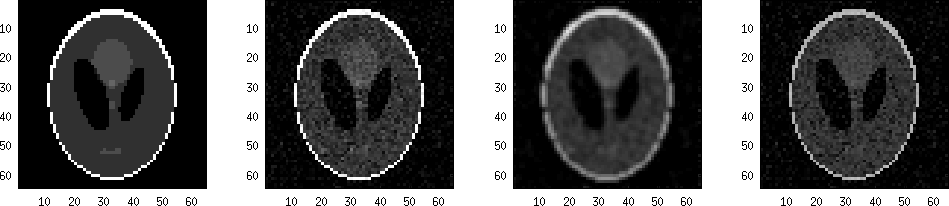
\includegraphics{noisey_images.png}

        \caption{\label{fig:images} {\it Left:} Original image. {\it Left
            middle:} Original image with added Gaussian noise. {\it Right
            middle:} Denoised image with a local kernel filter. {\it Right:}
        Denoised image with intensity matching.}

    \end{figure}

    \clearpage
    %\pythonexternal{hw2.m}
    Below is the code used to perform the intensity matching denoising.
    \lstinputlisting{hw2.m}

\end{homeworkProblem}
%===============================================================================



\end{document}

